\documentclass[aspectratio=169]{beamer}

\usepackage{subcaption}
\usepackage{emoji}

\title{Evaluación y desarrollo de \textit{eye tracking} remoto en navegadores
\textit{web}}
\author{Francisco Figari, Juan Kamienkowski, Gustavo Juantorena, Bruno Bianchi}
\date{Buenos Aires, 2022}
\titlegraphic{
\includegraphics[width=8em]{img/logo-fcen.png}}

\setbeamertemplate{navigation symbols}{}

% TODO: Hacer que esto sea opcional
\setbeamertemplate{frametitle}{
  \insertsectionhead\par
  \vspace*{0.2mm}
  \insertsubsectionhead\par
  \vspace*{0.2mm}
  \insertframetitle
}

\begin{document}

\frame{\titlepage}

\section{Introducción}

\begin{frame}{~}

  \begin{itemize}
      \item Los ojos son una ventana a los procesos cognitivos y estados
        emocionales de una persona
      \item Importante fuente de información que puede ser estudiada de manera
        no-invasiva
  \end{itemize}

  \begin{figure}
    \begin{subfigure}{0.49\textwidth}
      \centering
      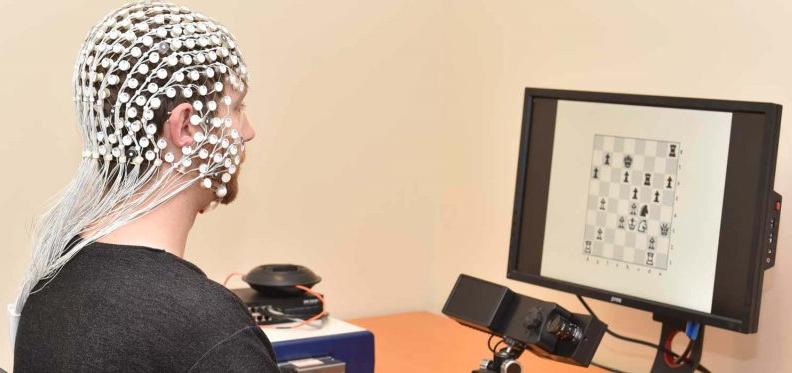
\includegraphics[width=\linewidth]{img/eye-link-eeg.jpg}
      \caption{\textit{Eye tracking} combinado con electroencefalograma}
    \end{subfigure}
    \begin{subfigure}{0.49\textwidth}
      \centering
      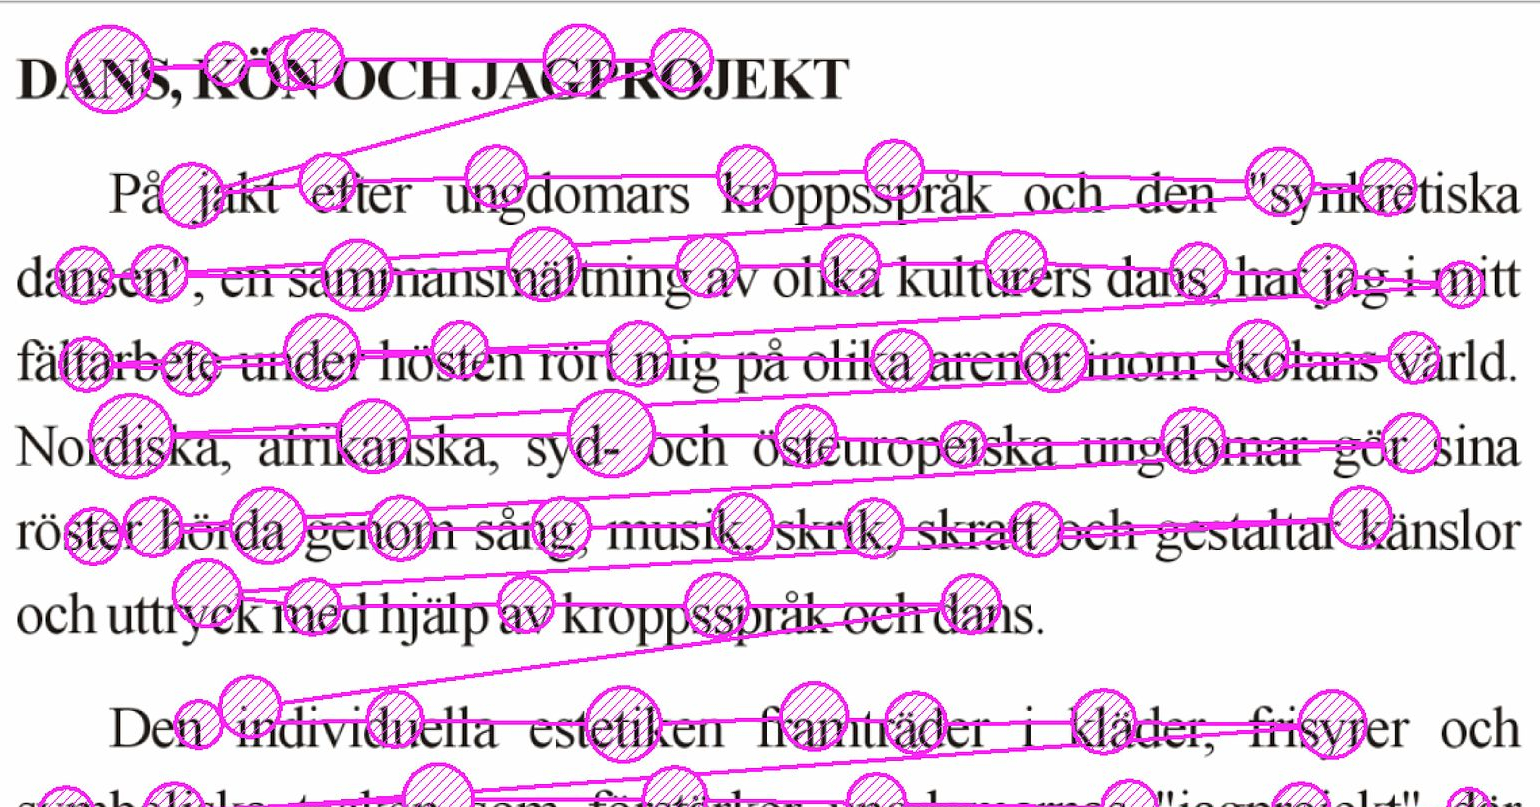
\includegraphics[width=\linewidth]{img/reading-fixations-saccades.jpg}
      \caption{Estimación de la mirada durante una tarea de lectura}
    \end{subfigure}
  \end{figure}

\end{frame}

\begin{frame}{\textit{Eye tracking} de laboratorio}

  \begin{columns}
    \begin{column}{0.5\textwidth}
      \begin{itemize}
        \item Consiste en estimar que posición de una pantalla está mirando el
          usuario
        \item Un \textit{stream} de frames de la webcam como \textit{input}
        \item Implica resolver: \begin{itemize}
            \item Localización de los ojos
            \item Estimación de la mirada
            \item Mecanismos de calibración
            \item Criterios de recalibración
        \end{itemize}
      \end{itemize}
    \end{column}

    \begin{column}{0.5\textwidth}
      \begin{figure}
        \centering
        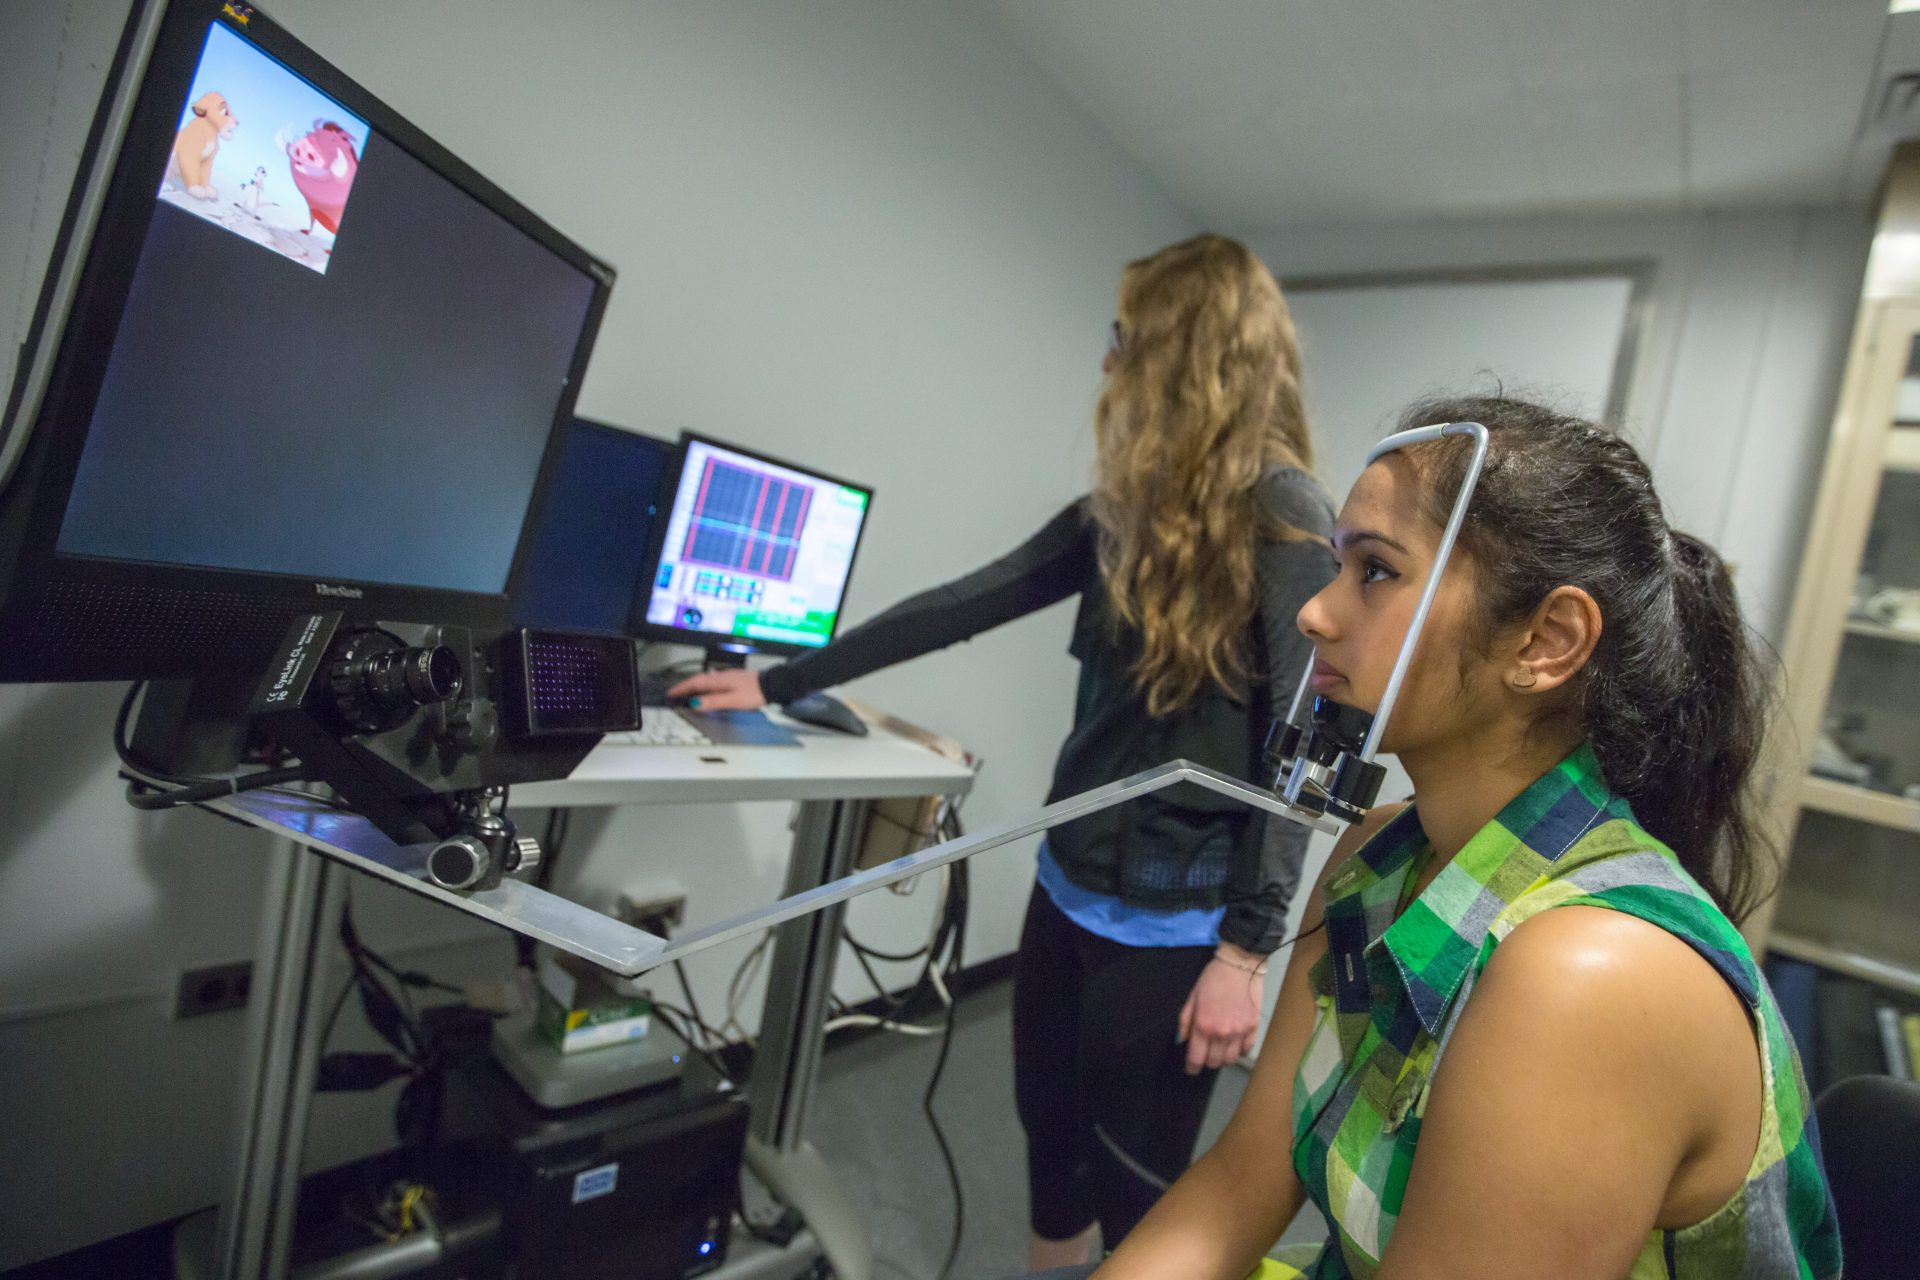
\includegraphics[width=\linewidth]{img/eye-link-chinrest.jpg}
        \caption{La reestricción de movimiento facilita mantener calibrado el
        sistema}
      \end{figure}
    \end{column}
  \end{columns}
\end{frame}

\begin{frame}{\textit{Eye tracking} de laboratorio}
  \begin{columns}
    \begin{column}{0.5\textwidth}
      \begin{itemize}
        \item Comunmente resuelto con sistemas comerciales cerrados
        \item Costos altos mientras que el hardware en sí representa una
          pequeña fracción de estos
        \item Imposibilidad de auditar la implementación
        \item Necesidad de asistir a un laboratorio
      \end{itemize}
    \end{column}

    \begin{column}{0.5\textwidth}
      \begin{figure}
        \centering
        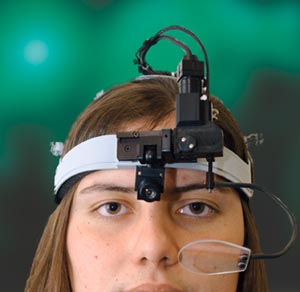
\includegraphics[width=0.8\linewidth]{img/eye-tracker-head-mounted.jpg}
        \caption{\textit{Eye tracker} montado a la cabeza}
      \end{figure}
    \end{column}
  \end{columns}
\end{frame}

\begin{frame}{\textit{Eye tracking} alternativo}

  \begin{columns}
    \begin{column}{0.4\textwidth}
      \begin{itemize}
        \item Interés en proveer software de \textit{eye tracking}

        \item Posibilidad de \textit{crowdsourcing}

          % e.g., detectar pérdidas de atención en clases masivas
        \item Potencial para nuevas aplicaciones
      \end{itemize}

    \end{column}
    \begin{column}{0.6\textwidth}

      \begin{figure}
        \begin{subfigure}{0.49\textwidth}
          \centering
          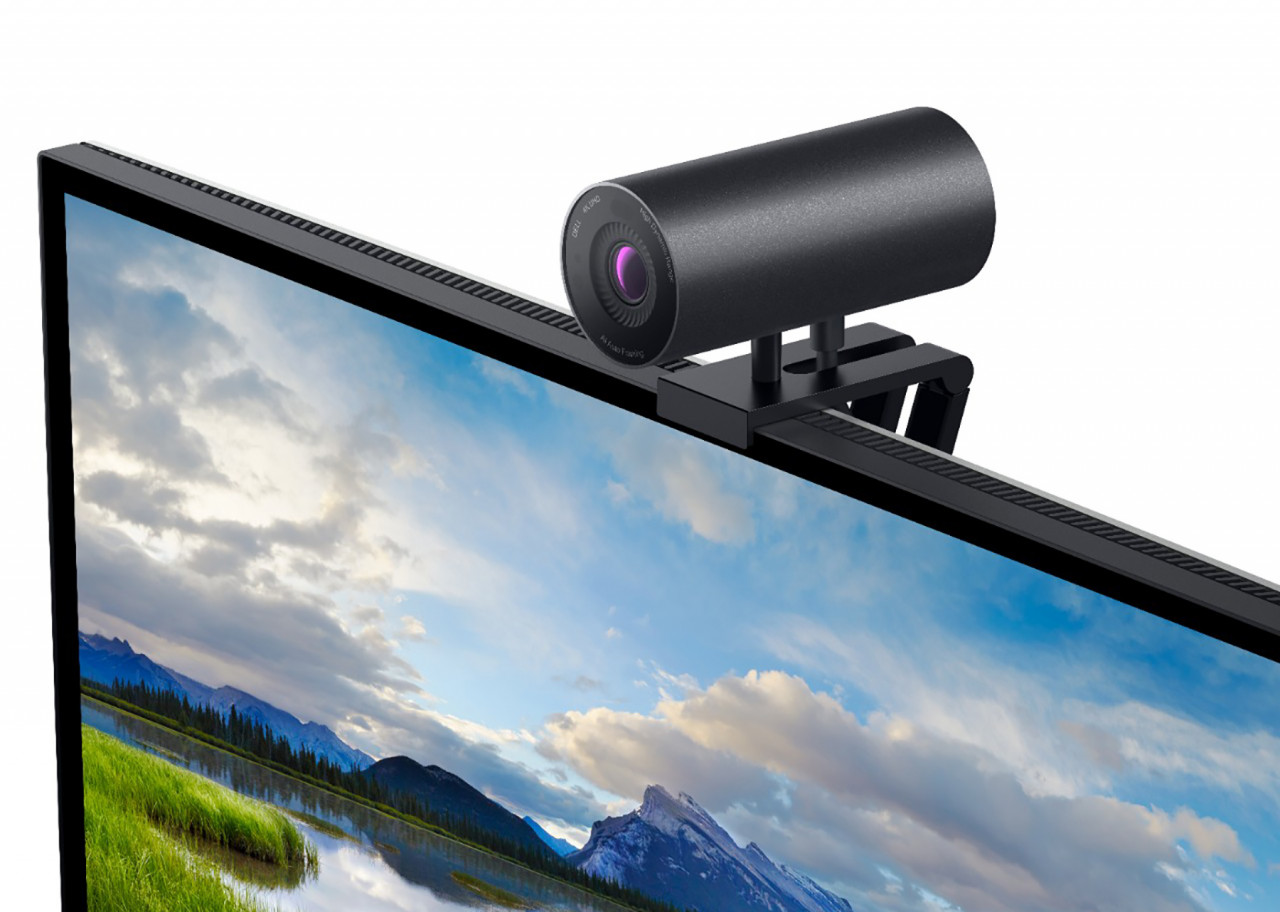
\includegraphics[width=0.8\linewidth]{img/external-webcam.jpg}
        \end{subfigure}
        \begin{subfigure}{0.49\textwidth}
          \centering
          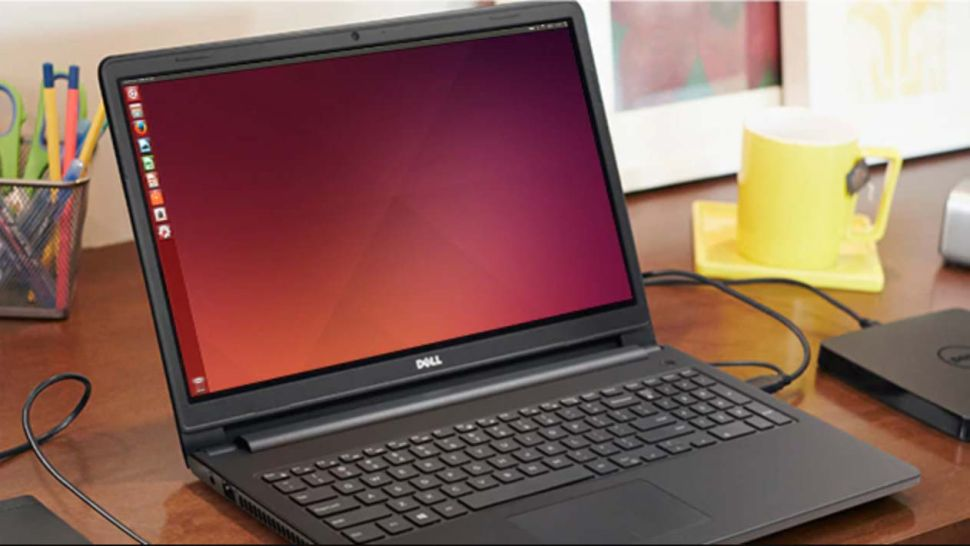
\includegraphics[width=0.8\linewidth]{img/notebook.jpg}
        \end{subfigure}
        \caption{Webcams domésticas ya disponibles}
      \end{figure}

      \begin{figure}
        \begin{subfigure}{0.49\textwidth}
          \centering
          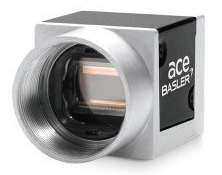
\includegraphics[width=0.6\linewidth]{img/basler-camera.jpg}
        \end{subfigure}
        \begin{subfigure}{0.49\textwidth}
          \centering
          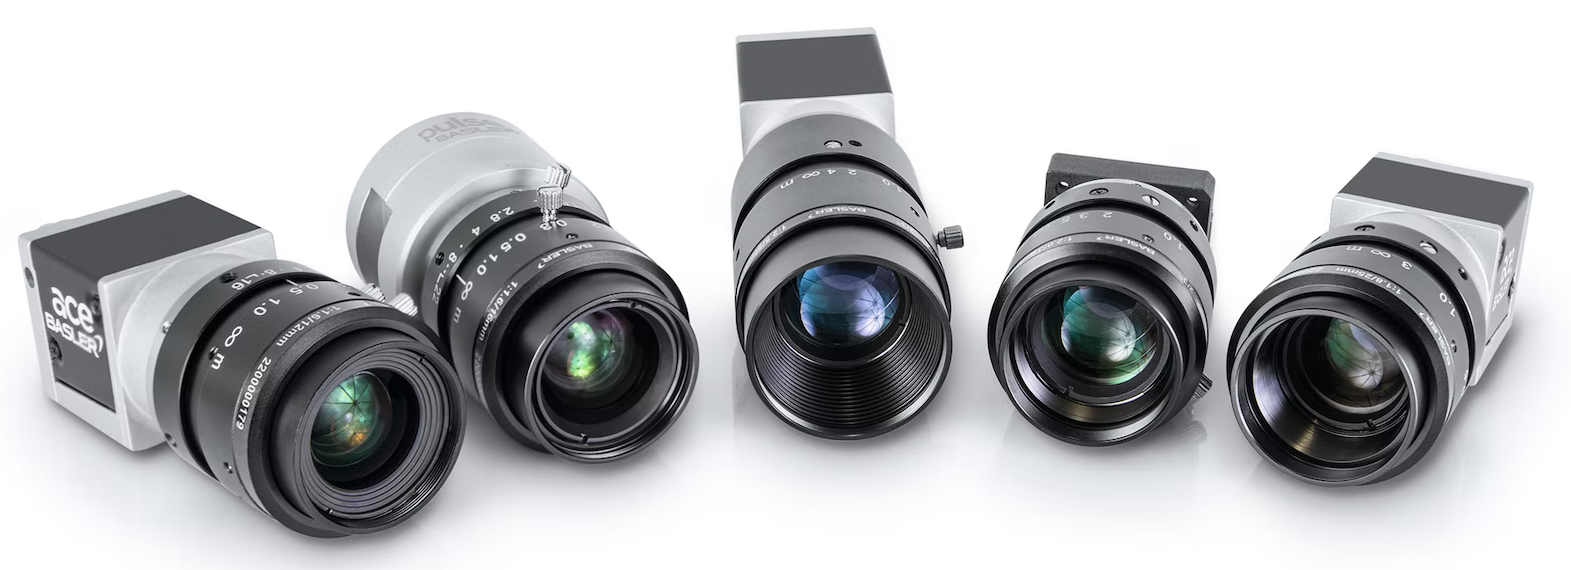
\includegraphics[width=0.8\linewidth]{img/basler-cameras-with-lens.png}
        \end{subfigure}
        \caption{Hardware profesional adquirible por una fracción del costo}
      \end{figure}

    \end{column}
  \end{columns}
\end{frame}

\begin{frame}{Implicancias del contexto remoto de navegador \textit{web}}

  \begin{itemize}
    \item[\emoji{thumbs-up}] Posibilidad de reutilizar cámaras web

    \item[\emoji{thumbs-up}] Compatibilidad con otras herramientas web, en
      particular \texttt{JSPsych}

    \item[\emoji{pinched-fingers}] Necesidad de implementar sobre
      \texttt{JavaScript}

    % no sólo las webcams son variables si no que tmb la compu donde corre el 
    % programa
    \item[\emoji{thumbs-down}] Hardware variable de potencialmente bajo rendimiento

    % deben transmitirse en texto e imagenes sin que puedan hacerse
    % aclaraciones en el momento. esto implica una duración total del
    % experimento potencialmente mayor
    \item[\emoji{thumbs-down}] Las instrucciones no pueden ser transmitidas en persona

    % puede variar la luz o la disposición del hardware
    \item[\emoji{thumbs-down}] Ambiente físico no controlado

    \item[\emoji{thumbs-down}] Limitados a una pequeña fracción de la
      bibliografía debido a tener una y sólo una cámara
  \end{itemize}

\end{frame}
\begin{frame}{Otros trabajos}
  \begin{columns}
    \begin{column}{0.5\textwidth}
      \begin{figure}
        \centering
        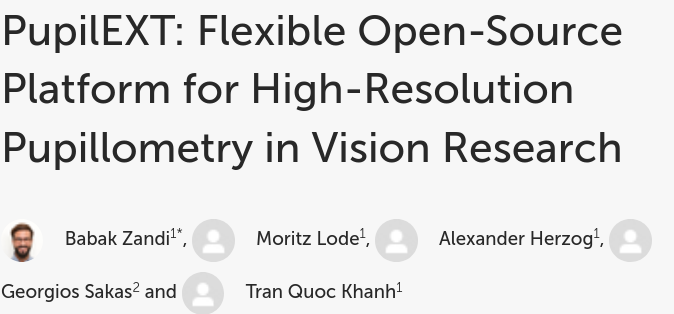
\includegraphics[width=0.8\linewidth]{img/pupil-ext.png}
        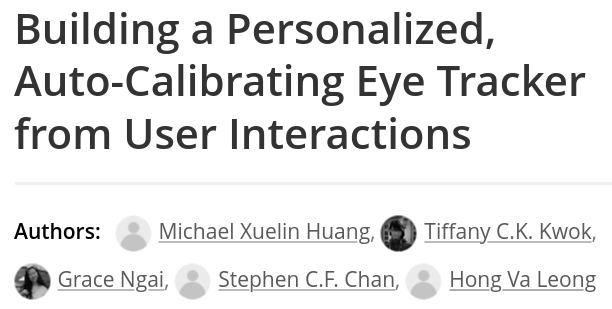
\includegraphics[width=0.8\linewidth]{img/PACE.png}
      \end{figure}
    \end{column}

    \begin{column}{0.5\textwidth}
      \begin{figure}
        \centering
        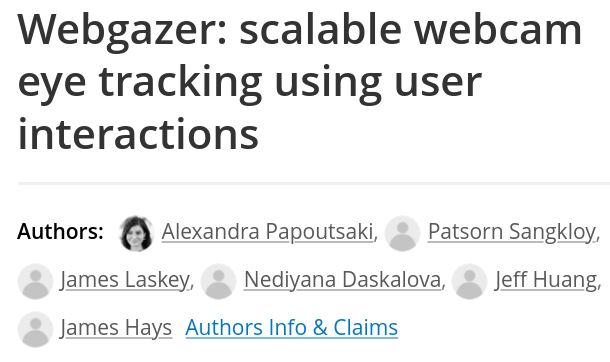
\includegraphics[width=0.7\linewidth]{img/webgazer.png}
        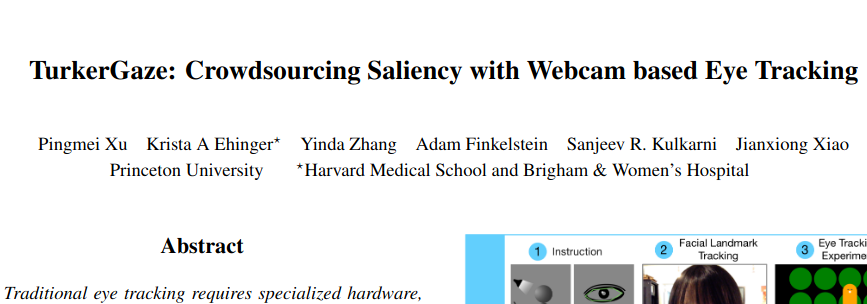
\includegraphics[width=\linewidth]{img/turker-gaze.png}
      \end{figure}
    \end{column}
  \end{columns}
  \begin{itemize}
    \item[\emoji{thumbs-down}] Falta de estándar respecto de cómo calibrar
    \item[\emoji{thumbs-down}] Ausencia de invarianza frente a movimientos de
      cabeza
  \end{itemize}
\end{frame}

\section{Objetivos}

\begin{frame}{~}

  \begin{itemize}
    \item Evaluar implementaciones recientes con similares motivaciones
    \item Implementar un prototipo de \textit{eye tracker} que corra en
      navegadores \textit{web}
    \item Establecer su capacidad en replicar conclusiones establecidas con
      \textit{eye trackers} tradicionales de laboratorio
  \end{itemize}
\end{frame}

\section{Implementación}

\begin{frame}{\texttt{WebGazer} como punto de partida}

  \begin{columns}
    \begin{column}{.5\textwidth}
      \begin{itemize}
        \item[\emoji{thumbs-up}] Extracción de \textit{frames} a través de la
          API del navegador
        \item[\emoji{thumbs-up}] Modelos de localización de los ojos y de
          estimación de la mirada
        \item[\emoji{thumbs-down}] Calibración inadecuada
        \item[\emoji{thumbs-down}] Ausencia de notificación de descalibraciones
        \item[\emoji{party-popper}] Corrregida falla de \texttt{WebGazer} que
          causaba \textit{crashes} del navegador en ciertas notebooks
      \end{itemize}
    \end{column}

    \begin{column}{.5\textwidth}
      \begin{figure}
        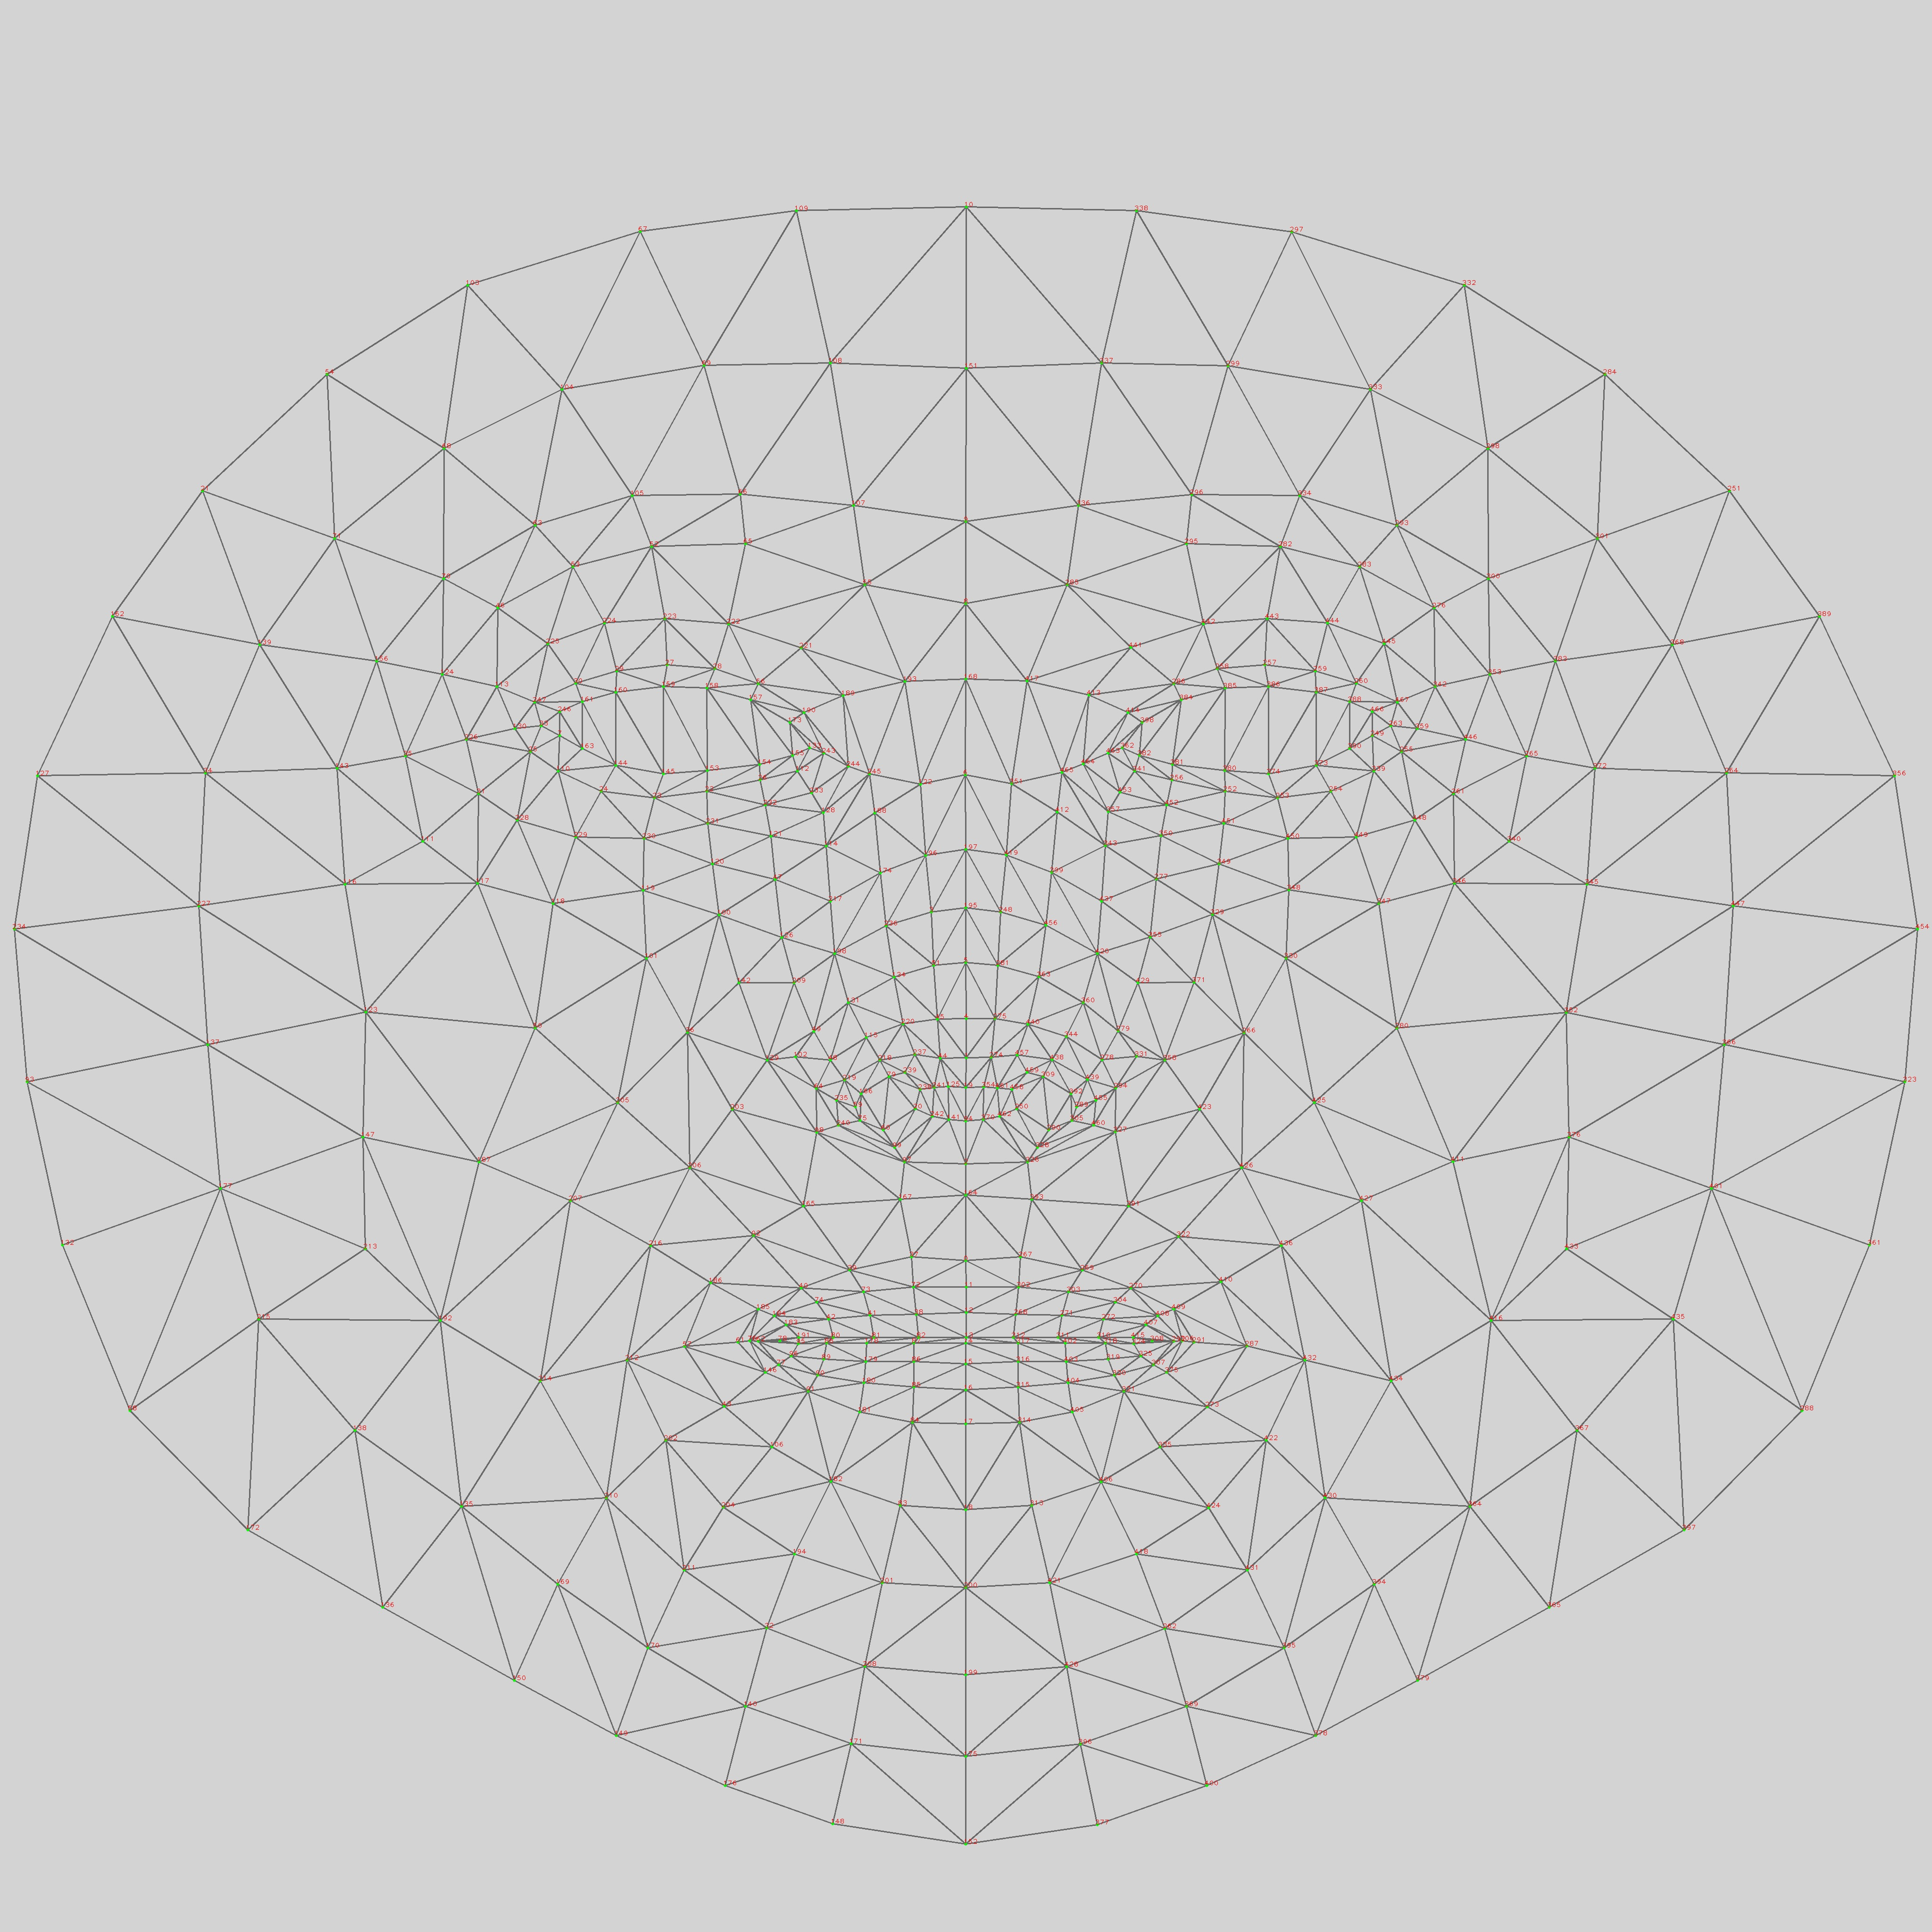
\includegraphics[width=0.75\linewidth]{img/facemesh-kepyoints.jpg}
        \caption{\textit{Output} del modelo de \textit{facemesh} utilizado por
        \texttt{WebGazer} para la localización de los ojos}
      \end{figure}
    \end{column}
  \end{columns}

\end{frame}

\begin{frame}{Calibración y validación}
  \begin{itemize}
    \item Nuestro caso de uso no garantiza interacciones

    \item Se muestran una serie de puntos, para cada uno de los cuales el
      usuario tendrá que fijar la mirada y presionar la barra de espacio
    
    \item Validación post calibración implementada de similar manera

    \item[\emoji{party-popper}] \texttt{WebGazer} adaptado para evitar cómputos
      ya no necesarios
  \end{itemize}
\end{frame}

\begin{frame}{Notificación de descalibración}

  \begin{columns}
    \begin{column}{.5\textwidth}
      \begin{itemize}
        \item Basada en detectar movimiento
        \item Instanciada luego de cada calibración
        \item Verificación realizada para cada \textit{frame}
        \item[\emoji{party-popper}] \texttt{WebGazer} adaptado para exponer los
          recuadros calculados en cada \textit{frame} por la rutina de
          localización de ojos
      \end{itemize}
    \end{column}

    \begin{column}{.5\textwidth}
      \begin{figure}
        \centering
        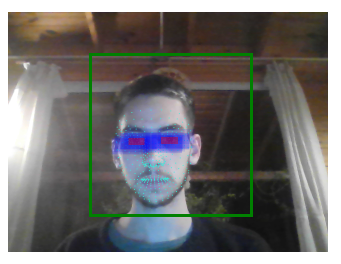
\includegraphics[width=\textwidth]{img/eyetracker-playground-screenshot.png}
        \caption{Detección de movimiento en funcionamiento}
      \end{figure}
    \end{column}
  \end{columns}

\end{frame}

\section{Experimentación}

\begin{frame}{Caso de estudio: tarea de antisacadas}

  \begin{columns}
    \begin{column}{.5\textwidth}
      \begin{itemize}
        \item Clínicamente relevante
        \item Resultados esperados ya establecidos
        \item Tarea simple para validar movimientos oculares
      \end{itemize}
    \end{column}
    \begin{column}{.5\textwidth}
      \begin{figure}
        \centering
        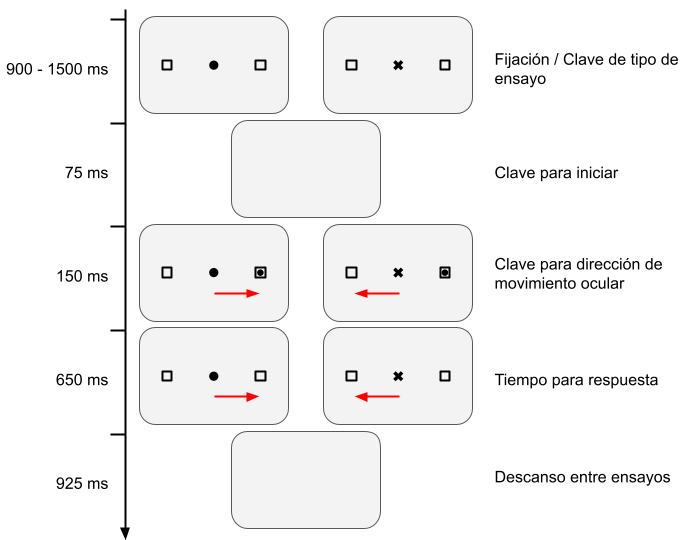
\includegraphics[width=\linewidth]{img/antisaccades-protocol.png}
        \caption{Protocolo de las tareas}
      \end{figure}
    \end{column}
  \end{columns}

\end{frame}

\begin{frame}{Primera instancia}
  \begin{itemize}
    \item Limitados a 10 minutos debido a una falla de \texttt{WebGazer}
    \item Únicamente ensayos de antisacada
    \item Recalibración luego de cada notificación de descalibración
    \item Sin validación post calibración
  \end{itemize}
\end{frame}

\begin{frame}{Segunda instancia}
  \begin{itemize}
    \item Duración superior a 20 minutos
    \item Ensayos de prosacadas y de antisacadas
    \item Recalibración cada 10 ensayos y sólo si se detectó una
      descalibración
    \item Con validación post calibración
  \end{itemize}
\end{frame}

\begin{frame}{Implementación y distribución}

  \begin{columns}
    \begin{column}{0.4\textwidth}
      \begin{figure}
        \centering
        
\includegraphics[width=\textwidth]{img/jspsych-logo.jpg}
      \end{figure}
    \end{column}
    \begin{column}{0.6\textwidth}
      \begin{figure}
        \centering
        
\includegraphics[width=0.8\textwidth]{img/cognition-run-logo.png}
        
\includegraphics[width=\textwidth]{img/neuropruebas-logo.jpg}
      \end{figure}
    \end{column}
  \end{columns}
\end{frame}


\section{Resultados}

\begin{frame}{Ejemplo de \textit{output} del sistema}
  \begin{figure}
    \centering
    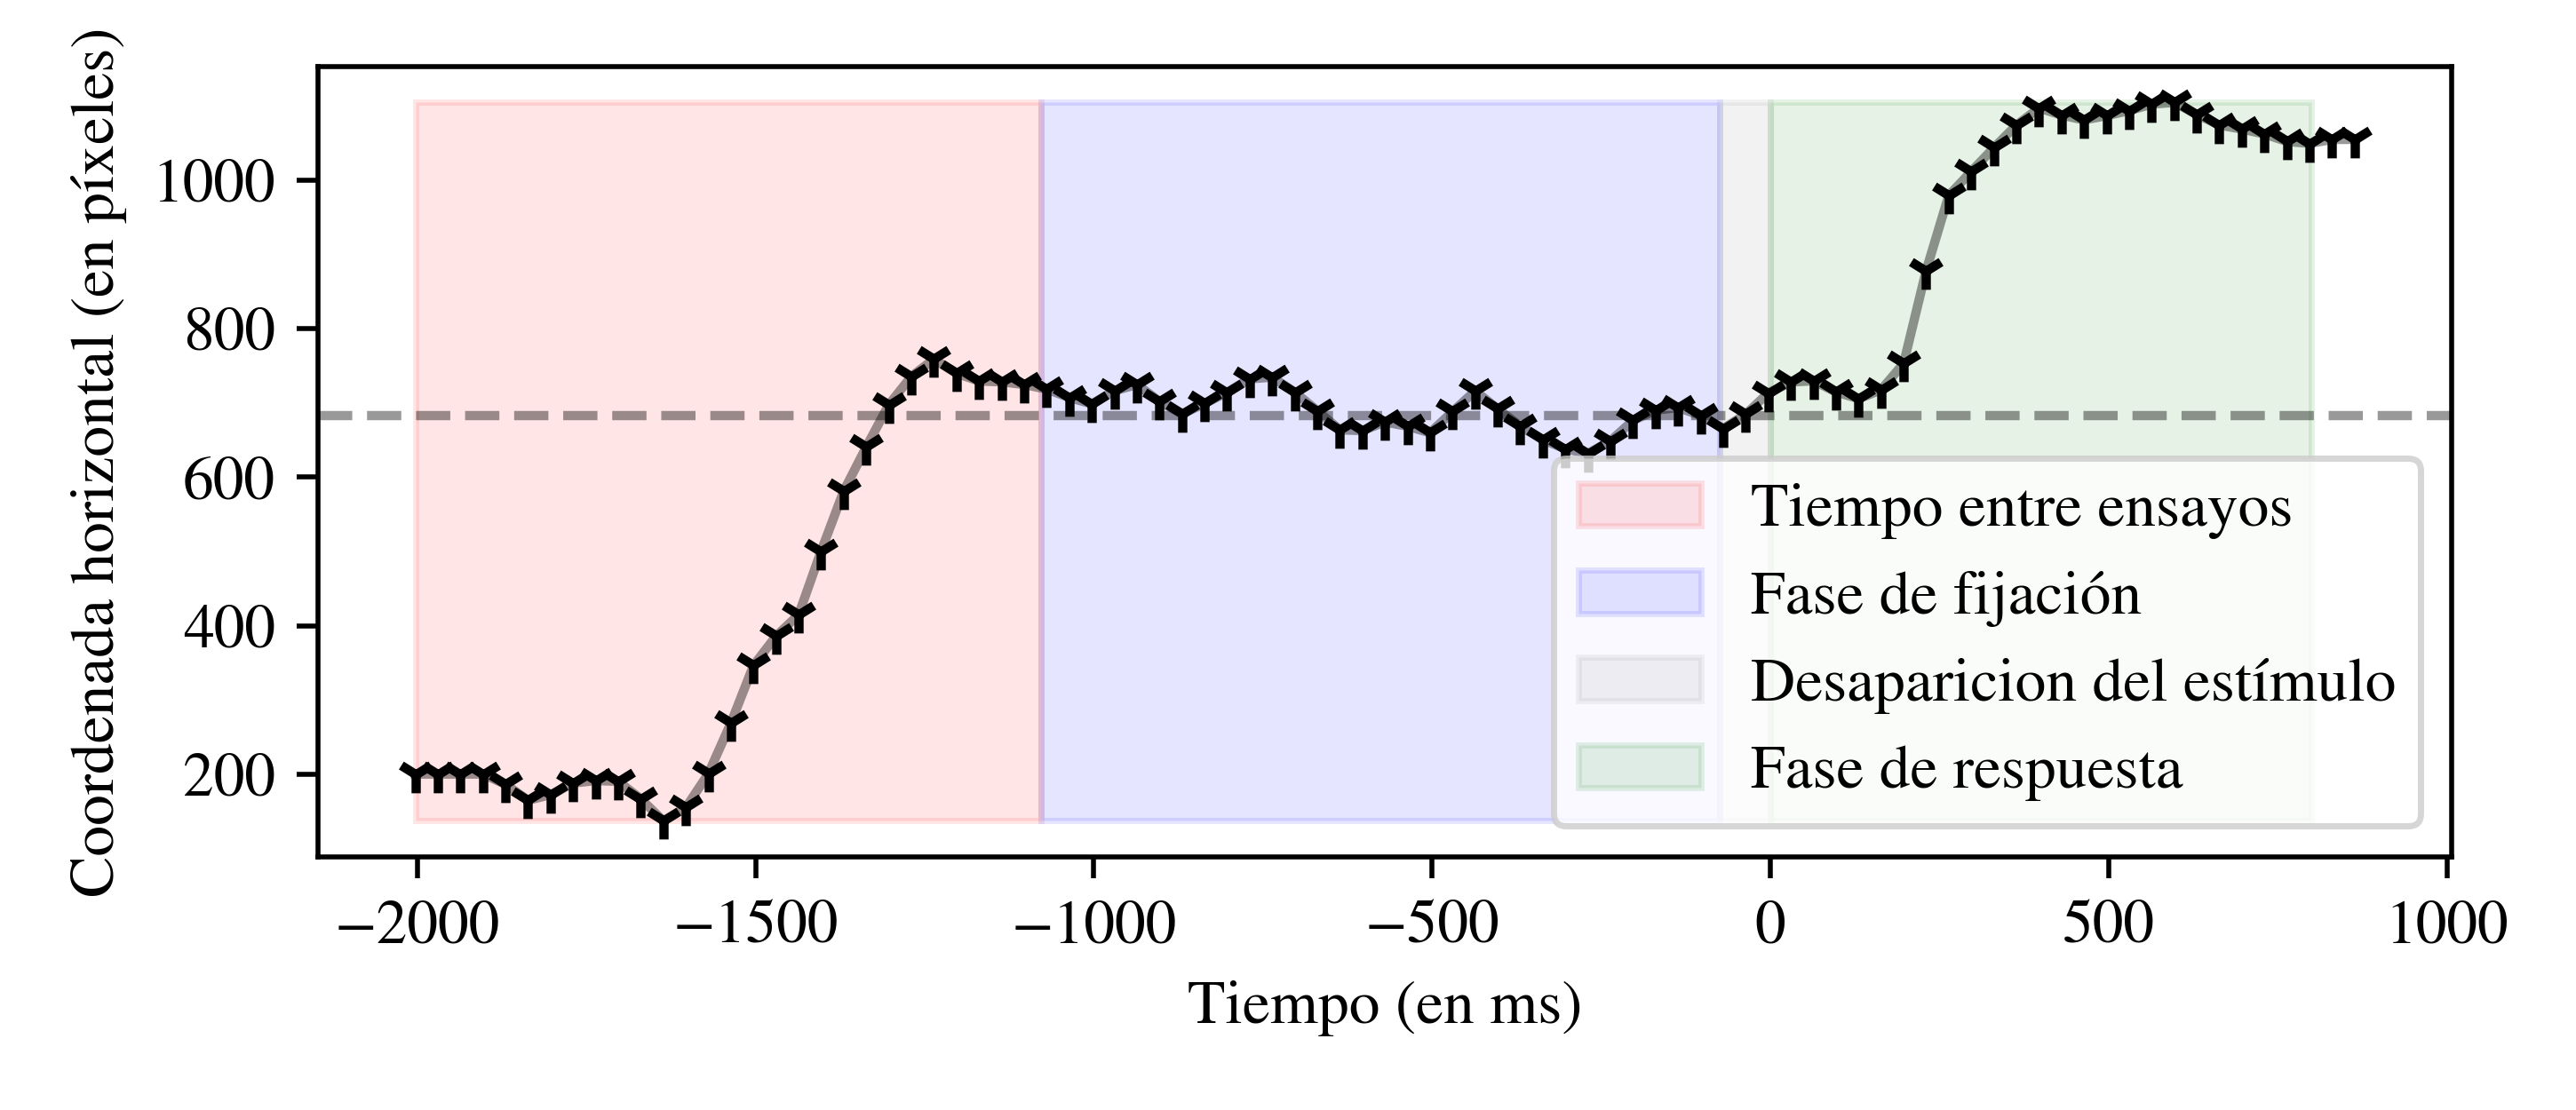
\includegraphics[width=\linewidth]{plots/output-example.png}
  \end{figure}
\end{frame}

\begin{frame}{Frecuencias de muestreo}
  \begin{figure}
    \centering
    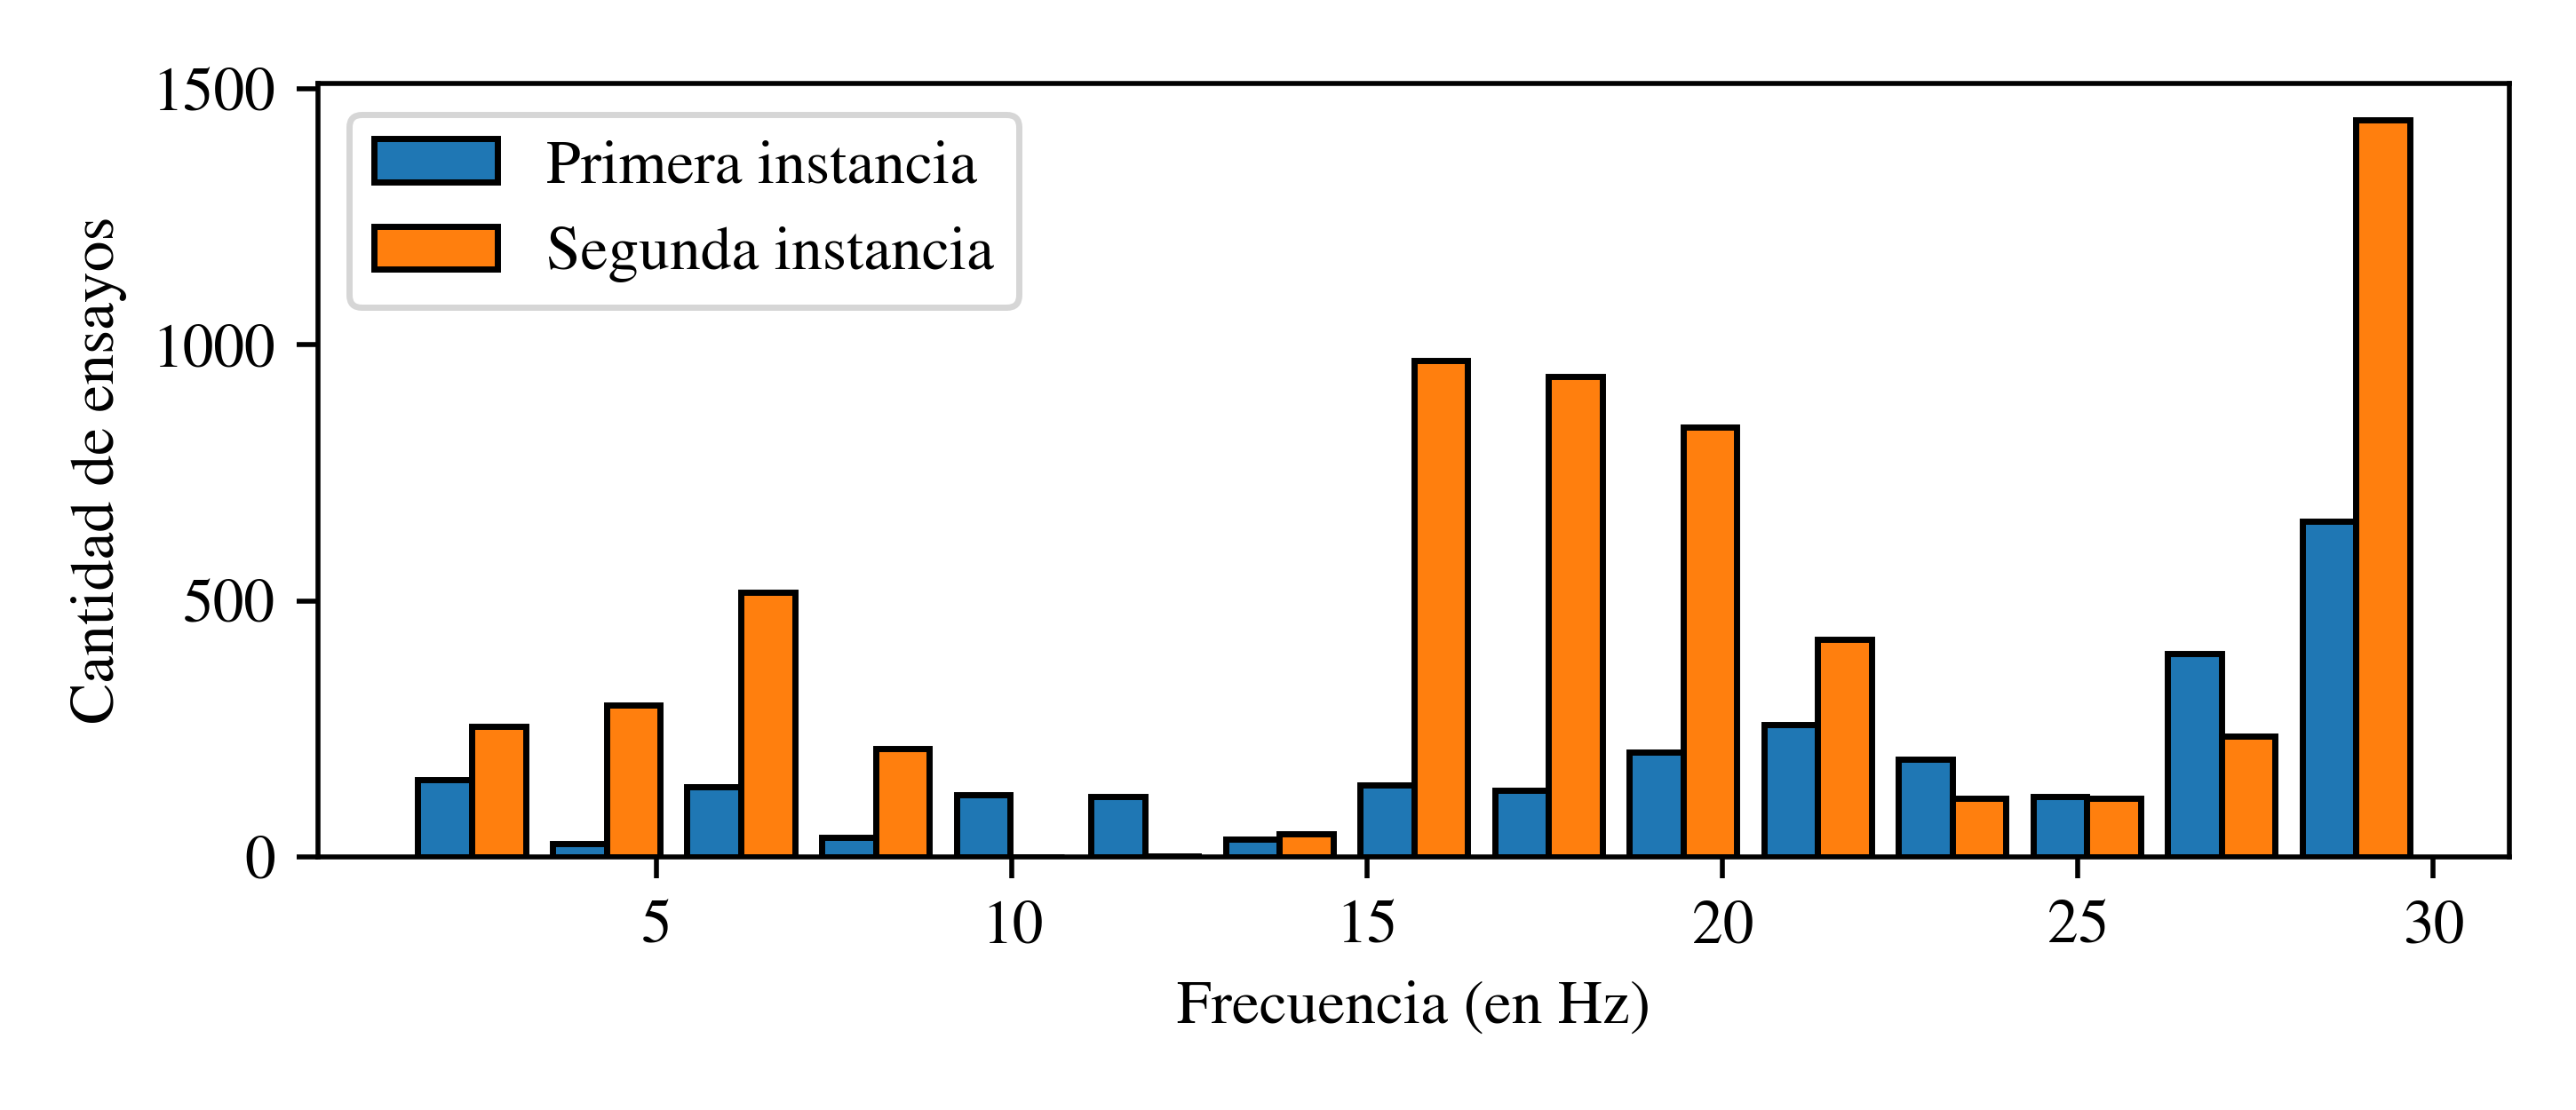
\includegraphics[width=\linewidth]{plots/sampling-frequencies-distribution.png}
  \end{figure}
\end{frame}

\begin{frame}{Anchos de pantalla}
  \begin{figure}
    \centering
    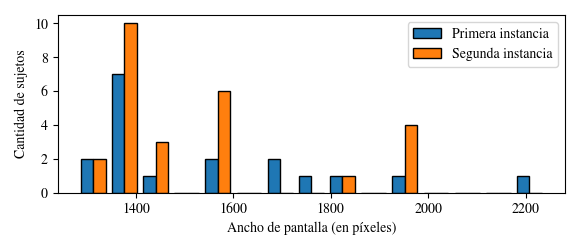
\includegraphics[width=\linewidth]{plots/screens-widths-distribution.png}
  \end{figure}
\end{frame}

\begin{frame}{Estimaciones desviadas}
  \begin{figure}
    \centering
    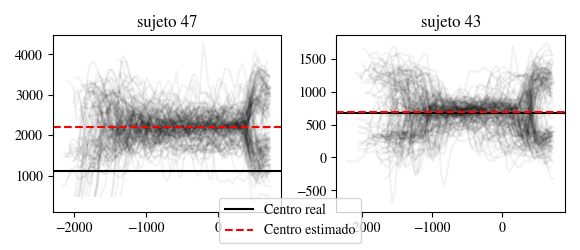
\includegraphics[width=\linewidth]{plots/skewed-estimations-examples.png}
    \caption{Las estimaciones de algunos sujetos están desviadas de los valores reales}
  \end{figure}
\end{frame}

\begin{frame}{Limpieza y normalización}
  \begin{columns}
    \begin{column}{0.4\textwidth}
      \begin{itemize}
        \item Ensayos descartados: \begin{itemize}
          \item frecuencia menor a 15 Hz
          \item a mano
          \item si el sujeto se distrajo de la tarea
        \end{itemize}
        \item Frecuencia de muestreo: \textit{Upsampling} a 30 Hz usando
          interpolación lineal
      \end{itemize}
    \end{column}
    \begin{column}{0.6\textwidth}
      \begin{figure}
        \centering
        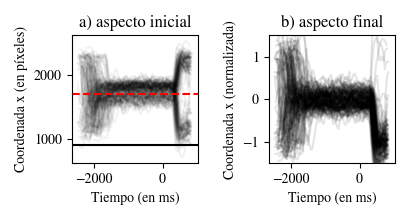
\includegraphics[width=\linewidth]{plots/normalization-example.png}
        \caption{Normalizado y espejado}
      \end{figure}
    \end{column}
  \end{columns}
\end{frame}

\begin{frame}{Detección de sacadas}
  \begin{columns}
    \begin{column}{0.5\textwidth}
      \begin{figure}
        \centering
        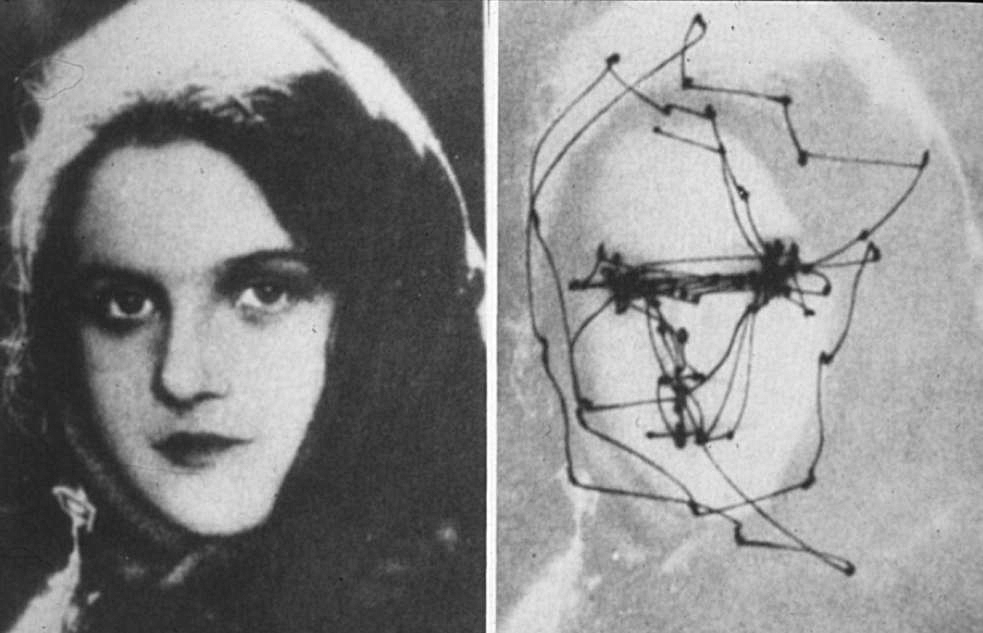
\includegraphics[width=\linewidth]{img/saccades-example.jpg}
        \caption{Los movimientos oculares muestran qué elementos de una imagen
        capturan la atención}
      \end{figure}
    \end{column}
    \begin{column}{0.5\textwidth}
      \begin{figure}
        \centering
        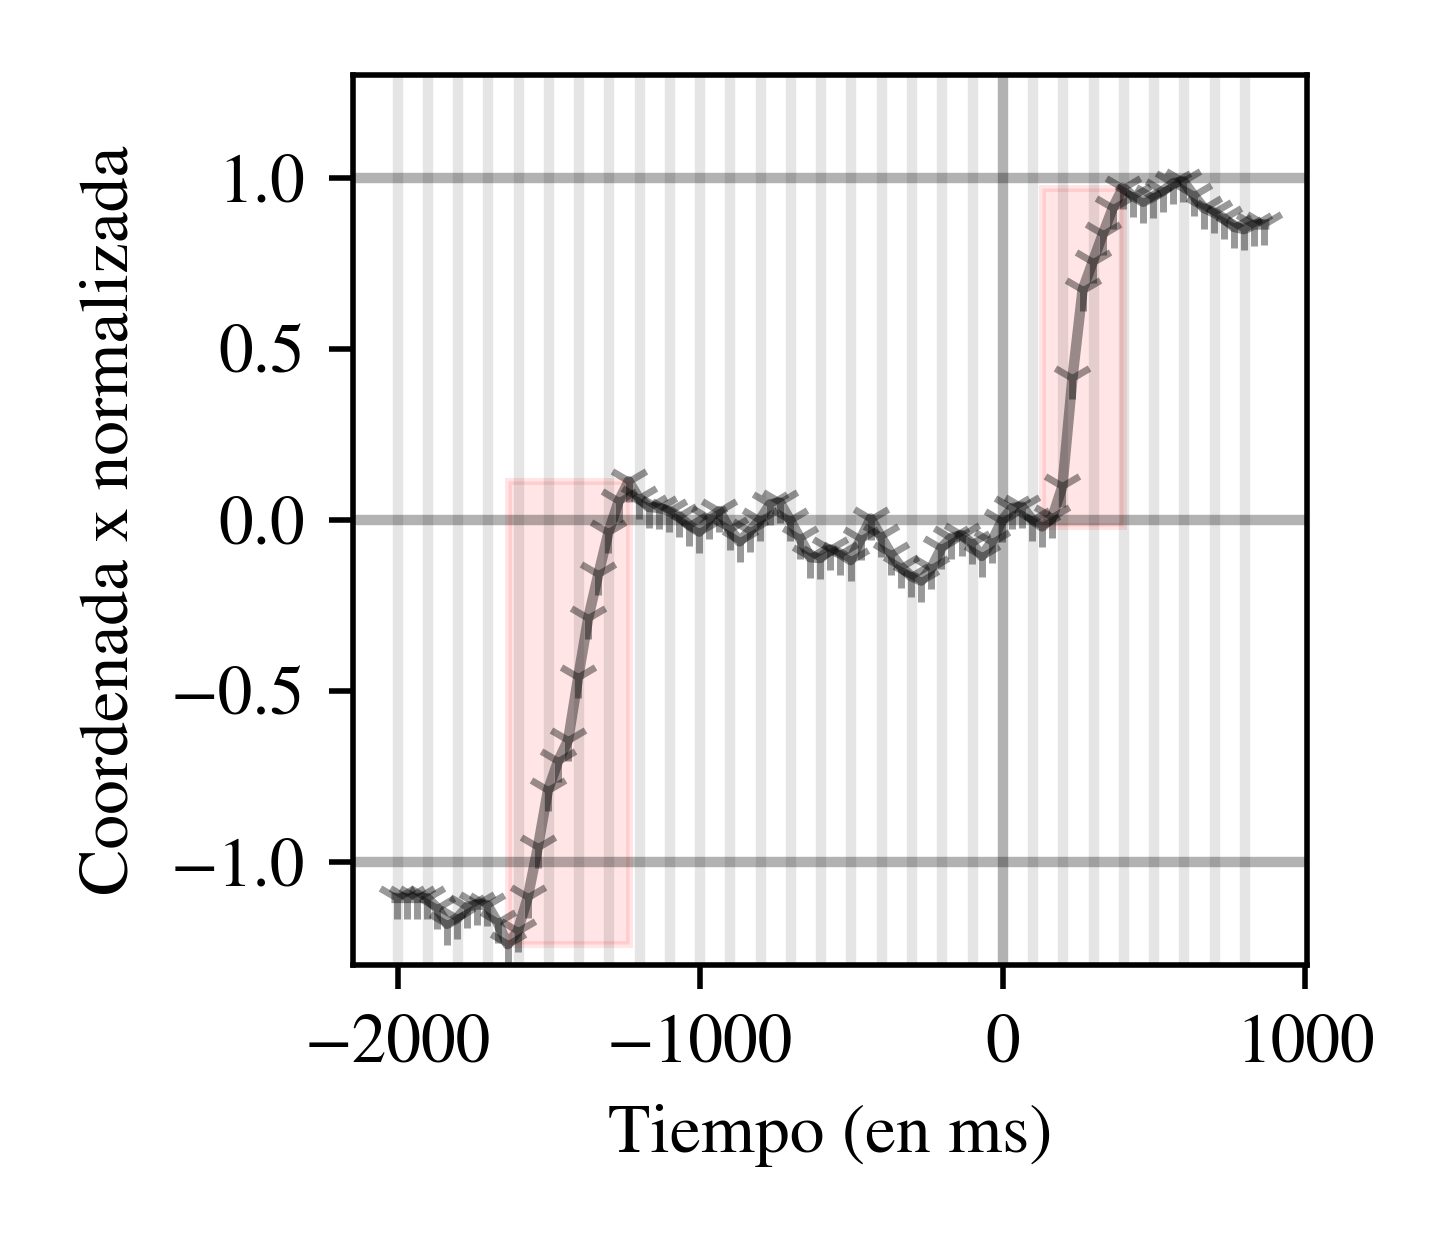
\includegraphics[width=\linewidth]{plots/detected-saccades-example.png}
        \caption{Sacadas detectadas sobre las estimaciones de un ensayo}
      \end{figure}
    \end{column}
  \end{columns}
\end{frame}

\begin{frame}{Conclusiones generales replicadas}
  \begin{table}
    \centering
    \begin{tabular}{ l | c | c | c }
      & correctitud & \multicolumn{2}{ c }{tiempo de respuesta (ms)} \\
      &             & correcto & incorrecto \\
      \hline
      antisacada & 81.29\% & 509 (93) & 346 (105) \\
    \end{tabular}
    \caption{Primera instancia}
  \end{table}
  
  \begin{table}
    \centering
    \begin{tabular}{ l | c | c | c }
      & correctitud & \multicolumn{2}{ c }{tiempo de respuesta (ms)} \\
      &             & correcto & incorrecto \\
      \hline
      antisacada & 94.82\% & 358 (109) & 299 (103) \\
      \hline
      prosacada & 98.09\% & 320 (108) & 311 (150) \\
    \end{tabular}
    \caption{Segunda instancia}
  \end{table}

  \emoji{thumbs-down} En la bibliografía para la tarea de antisacadas se
  reportan \textbf{valores de correctitud} más cercanos al rango $[60\%,
  75\%]$.
\end{frame}

\begin{frame}{Menos datos de lo esperado}
  \begin{columns}
    \begin{column}{0.4\textwidth}
      \begin{itemize}
        \item Cantidad de ensayos iniciales baja en relación a otros trabajos
        \item Descarte de aproximadamente $\frac{2}{3}$ de los datos
        \item Altas e inesperadas tasas de correctitud
      \end{itemize}
    \end{column}

    \begin{column}{0.6\textwidth}
      \begin{table}
        \centering

        \begin{tabular}{ l | c | c }
          Antisacadas   & incorrecto  & correcto \\
          \hline
          \# total      & 64          & 1173 \\
          \hline
          \# por sujeto & 4.57 (2.84) & 78.20 (40.38)
        \end{tabular}

        \vspace{0.3cm}

        \begin{tabular}{ l | c | c }
          Prosacadas    & incorrecto  & correcto \\
          \hline
          \# total      & 22          & 1134 \\
          \hline
          \# por sujeto & 2.44 (1.23) & 75.59 (38.58)
        \end{tabular}

        \caption{Desbalance entre grupos incorrecto y grupo correcto}
      \end{table}
    \end{column}
  \end{columns}
\end{frame}

\section{Conclusiones}

\begin{frame}{~}
  \begin{itemize}
    \item Campo aún en sus primeros pasos
    \item Se obtuvo un prototipo de \textit{eye tracker} para navegadores web
    \item Potencial para realizar análisis clínicos remotos
    \item Precisión muy por debajo de aquella alcanzable por \textit{eye
      trackers} profesionales
  \end{itemize}
\end{frame}

\subsection{Limitaciones}

\begin{frame}{Implementativas}
  TODO: Las limitaciones y trabajo futuro no ponerlas todas y en cambio referir
  a la tesis \par

. bajas frecuencias
. pestañeos
. estimación del tamaño de la pantalla
. imprecisión en la duración de cada frame, problemático si se quiere mostrar
  un estímulo durante una corta duración de tiempo

  \begin{figure}
    \centering
    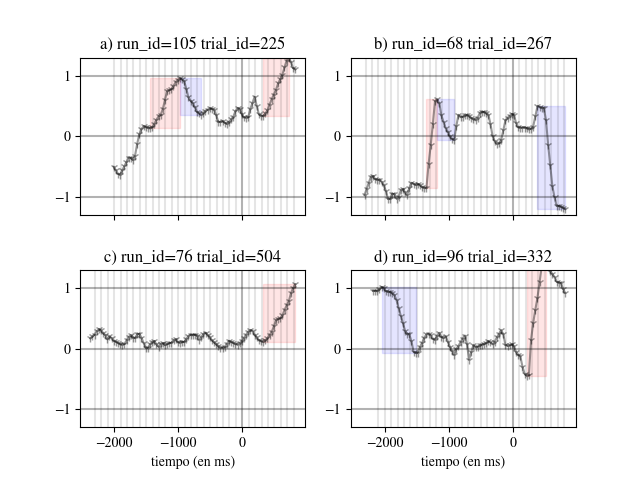
\includegraphics[width=0.9\linewidth]{img/undetected-saccades-examples.png}
    \caption{Ejemplos de sacadas no detectadas}
  \end{figure}
\end{frame}

\begin{frame}{Experimentales}
. proporción de datos filtrados demasiado elevada
. necesidad de revisar la causa de las altas tasas de correctitud obtenidas
. representatividad de distintos grupos etarios
\end{frame}

\subsection{Trabajo futuro}

\begin{frame}{Análisis de datos}
. Investigar e implementar mecanismos estándares de detección de sacadas, lo
  cual podría basarse en la previa construcción de un dataset etiquetado de
  sacadas
. Revisar criterios de exclusión para asegurarse de no estar filtrando datos
  válidos
. Realizar nuevas rondas de experimentación, estimando previamente la cantidad
  de ensayos necesarios para asegurar cantidades suficientes en los grupos
  incorrectos y en los distintos grupos etarios
\end{frame}

\begin{frame}{Análisis de sensibilidad}
. propuesta sobre experimento para recolectar datos y establecer métricas de
  calidad sobre las estimaciones obtenidas por la herramienta
TODO: Acá combinar un poco lo que quedó en la tesis y lo que pensé para
      sensitivity analysis
\end{frame}

\begin{frame}{Prototipo desarrollado}
. optimizar frecuencia de muestreo
. reexplorar detección de descalibraciones y qué significa que el sistema esté
  descalibrado
. mejorar la calibración, generalizarla a más puntos de interés
. detección de pestañeos
. estimación del tamaño de la pantalla y posibilidad de mostrar estímulos en
  grados
. verificación de condiciones iniciales
TODO: Extender con lo que haya escrito en la tesis
\end{frame}

\begin{frame}{\textit{Eye tracking} en navegadores \textit{web}}
. extender bibliografía que aplique a nuestro contexto
. eye tracking web no podría atacar algunos problemas que sí puede el eye
  tracking tradicional, pero al ser remoto y de bajo costo es posible que
  permita atacar nuevos problemas. Deben entonces buscarse tales problemas
\end{frame}

\end{document}
